\documentclass{article}
\usepackage{graphicx}
\usepackage{amsmath}   
\usepackage{amsthm}
\usepackage{amsfonts} 
\usepackage{tikz}
\usepackage{pgfplots}
\usepackage{parskip}
\pgfplotsset{compat=1.18}
\setlength{\parindent}{0pt}
\renewcommand{\baselinestretch}{1.3}

% Macros 
\newcommand\bfrac[2]{\frac{\displaystyle #1}{\displaystyle #2}}

\title{05-S1-Q4 \\ Solution + Discussion}
\author{David Puerta}
\date{}

\definecolor{BLUE}{RGB}{101,149,179}

\newcommand{\der}[2]{\frac{\mathrm{d}#1}{\mathrm{d}#2}}

\begin{document}

\maketitle

\begin{abstract}
    \noindent In this document we will go through the solution to the 05-S1-Q4 question and provide a discussion of the question at the end. There are also hints on the first page to aid you in finding a solution. There is no single method that results in an answer to a STEP question, there are a multitude of different paths that end up at the same solution. However, some methods are more straight forward and you are encouraged to take the path of least resistance.  
\end{abstract}

\vspace{1cm}

\begin{center}
    \textbf{Hints}
\end{center}

\textbf{(a)}: Is $\sin \theta$ positive or negative in the region $3\pi /2 \leq \theta \leq 2\pi$? 

\vspace{1cm}

\textbf{(b)}: Can you find any rational roots to the cubic in $\tan \theta$? How many solutions are there to $\tan 3\theta=11/2$ for $\pi/4 \leq \theta \leq \pi/2$?



\newpage

\begin{center}
    \textbf{Solution}
\end{center}

\vspace{0.5cm}

\textbf{(a)} Sketching both $\sin x$ and $\cos x$ in the required region

\begin{figure}[h!]
\centering
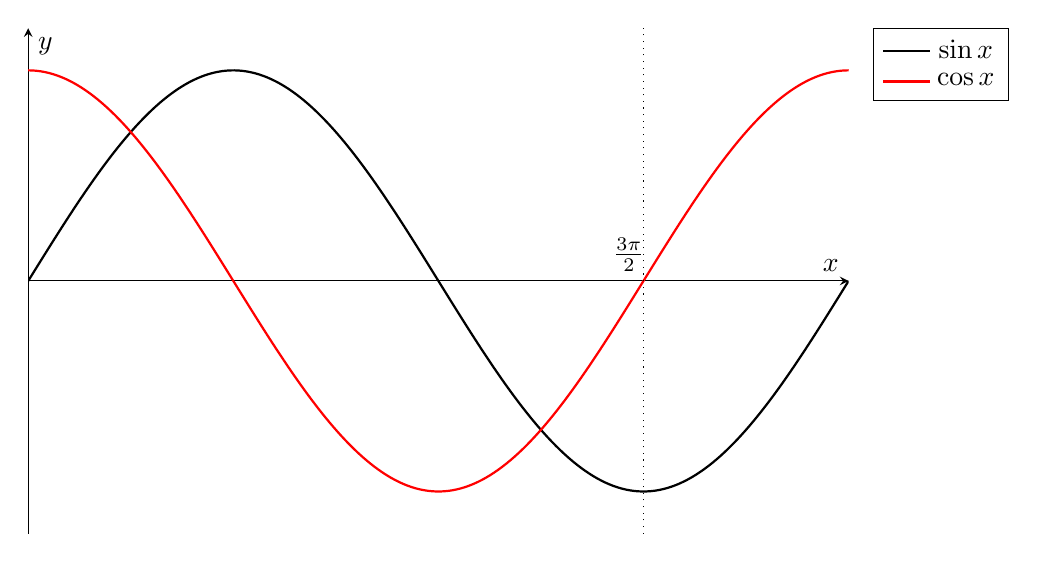
\begin{tikzpicture}[scale=1]
  \begin{axis}[
    axis lines=middle,
    xmin=0, xmax=6.283185307,
    ymin=-1.2, ymax=1.2,
    samples=200,
    xlabel={$x$},
    ylabel={$y$},
    domain=0:6.283185307,
    ticks=none,
    width=12cm,
    height=8cm,
    legend pos=outer north east
  ]
    \addplot[black, thick] {sin(deg(x))};
    \addplot[red, thick]  {cos(deg(x))};
    \legend{$\sin x$,$\cos x$}

    \draw[dotted] (4.7124,-1.2) -- (4.7124,1.2);
    \node[above] at (4.6,0) {$\frac{3\pi}{2}$};
    
  \end{axis}
\end{tikzpicture}
\end{figure}

we see that $\sin x$ is negative in the region $\frac{3\pi}{2} \leq \theta \leq 2\pi$.\par

Finding the value for $\sin x$ using the triangle (or using $\sin^2 x + \cos^2 =1$)
\begin{figure}[h!]
    \centering
        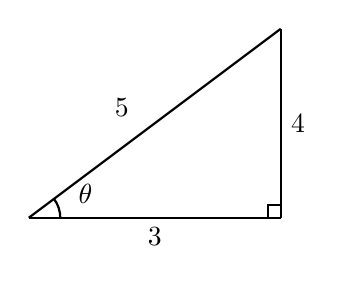
\begin{tikzpicture}[scale=0.8]
            \coordinate (O) at (0, 0);
            \coordinate (C) at (4, 0);
            \coordinate (P) at (4, 3);

            \draw[thick] (O) -- (C) node[midway, below] {\(3\)};
            \draw[thick] (C) -- (P) node[midway, right] {\(4\)};
            \draw[thick] (P) -- (O) node[midway, left, xshift=-2mm, yshift=2mm] {\( 5\)};

            \draw[thick] (3.8,0) -- (3.8,0.2) -- (4,0.2);

            \draw[-,thick] (0.5,0) arc[start angle=0, end angle=37, radius=0.5];
            \node[above] at (0.9,0.07) {\( \theta \)};

        \end{tikzpicture}
\end{figure}
and then taking the negative yields $\sin x=-\frac{4}{5}$. 

Finally, using the identity $\sin 2x =2\sin x\cos x$ gives 
\[
\sin2\theta=2\sin\theta \cos\theta=-2\cdot\frac{4}{5}\cdot\frac{3}{5}=-\frac{24}{25}.
\]

Using the compound angle formula for $\cos x$ 
\begin{equation}
    \cos(A \pm B) = \cos A \cos B \mp \sin A\sin B
\end{equation}
to give us the double angle formula for $\cos x$ as
\[
\cos 2x = \cos^2x - \sin^2x
\]
which using our values of $\sin\theta$ and $\cos \theta$ gives 
\[
\cos 2\theta = \left(\frac{3}{5}\right)^2 - \left(-\frac{4}{5}\right)^2 = -\frac{7}{25}.
\]
Substituting $A= 2\theta$ and $B=\theta$ in (1) gives
\[
\cos(2\theta +\theta) = \cos 3\theta = \cos 2\theta \cos \theta - \sin 2\theta\sin \theta
\]
which by our previous work gives 
\[
\cos 3\theta = \left(-\frac{7}{25}\right)\left(\frac{3}{5}\right) - \left(-\frac{24}{25}\right)\left(-\frac{4}{5}\right) = -\frac{117}{125}.
\]
\textbf{(b)} Recalling the compound angle formula for $\tan x$,
\begin{equation}
    \tan(A\pm B) = \frac{\tan A \pm \tan B}{1\mp\tan A\tan B}
\end{equation}
gives us the double angle formula for $\tan x$ as
\[
\tan2x=\frac{2\tan x}{1-\tan^2x}.
\]

Substituting $A=2\theta$ and $B=\theta$ in (2) gives 
\[
\tan(2\theta + \theta) = \tan 3\theta = \bfrac{\tan\theta + \frac{2\tan x}{1-\tan^2x}}{1-\tan\theta \frac{2\tan x}{1-\tan^2x}} = \frac{3\tan \theta - \tan^3 \theta}{1-3\tan^2\theta}.
\]

Using $\tan 3\theta = \frac{11}{2}$ and letting $\tan \theta = t$, the above triple angle formula gives
\[
\frac{11}{2} = \frac{3t - t^3}{1-3t^2} \Leftrightarrow 2t^3-33t^2-6t+11=0
\]
which we can check (Rational Root Theorem) has a rational root $t=1/2$. Hence, we can factor our cubic into 
\[
(2t-1)(t^2-16t-11)=0
\]
which gives three solutions for $t=\tan \theta$,
\[
\tan \theta = \frac{1}{2}, \quad \tan\theta = 8+5\sqrt{3}, \quad \tan \theta =8-5\sqrt{3}.
\]

\newpage

Sketching the graph of $\tan 3x$ for $0 \leq x \leq \pi/2$

\begin{figure}[h!]
\centering
    \includegraphics[width=0.5\linewidth]{Graph.png}
\end{figure}
we see that there are two solutions to $\tan 3x = 11/2$, the second one being the solution in our region $\pi/4 \leq \theta \leq \pi/2$. As $\tan x$ in strictly increasing on the interval $0 \leq x \leq \pi/2$, then we must have 
\[
\tan \theta = 8+5\sqrt{3}.
\]

\newpage

\begin{center}
    \textbf{Discussion}
\end{center}

\vspace{0.5cm}

Part (a) is quite straight forward, using the double angle formula for $\sin 2x$ then using the appropriate values for $\sin x$ and $\cos x$. Finding the correct value of $\sin x$ can be done using the triangle method (used in the provided solution) or solving 
\[
\sin^2\theta + \cos^2\theta = \sin^2 \theta + \left(\frac{3}{5}\right)^2 = 1 \Rightarrow \sin x = \pm \frac{4}{5}
\]
and taking the negative solution - both methods are completely valid. It is useful to note that we chose the correct value of $\sin x$ with the aid of a sketch of the function in the appropriate region to determine its sign. This will be used again in part (b) with an extra step.\par

Part (b) involves two parts. The first part is simple enough, substituting the double angle formula into the compound angle formula and simplifying gives the desired result. The second part requires some additional thinking, using the given value of $\tan3\theta=11/2$ and letting $\tan \theta = t$ (this is not necessary but it helps for clarity) gives a cubic
\[
2t^3-33t^2-6t+11=0
\]
which we can factorise by first looking for rational roots; this is done using the Rational Root Theorem.\par 

The Rational Root Theorem is useful anytime you are given a cubic, or higher degree polynomial, and there are no obvious solutions. Typically, if you are given a polynomial or degree three or higher (without a calculator) it will have rational roots. The theorem goes as follows.

If you have a polynomial
\[
a_nx^n+a_{n-1}x^{n-1}+\cdots+a_1x+a_0=0
\]
with $a_1,\cdots,a_n$ constants and $a_n \ne 0$, then this polynomial has a \textit{possible} rational root $x=\frac{p}{q}$ with $q$ a factor of $a_n$ and $p$ a factor of $a_0$.\footnote{You can restate this with $p$ and $q$ having a greatest common multiple of $1$ to ensure that the fraction you get cannot be reduced. This theorem can also be proven with not much effort so I challenge you to prove this using divisibility!} 

For example, for our polynomial 
\[
2t^3-33t^2-6t+11=0
\]
we see that if we have a rational root $x=\frac{p}{q}$ then the possible values of $p$ and $q$ are
\[
p = \pm 1 , \pm 11 \quad \text{and} \quad q=\pm1,\pm2
\]
remembering that negatives are also factors. Using trial and error, we spot that $x=1/2$ is indeed a solution.

Notice that the Rational Root Theorem states a \textit{possible} rational root, but does not guarantee a rational root. This theorem is quite useful anytime you are without the help of a calculator and I strongly recommend you have it in your arsenal. 

The final part of the question is seeing that we have two possible values of $\theta$ for which $\tan 3\theta =11/2$ and three values from our cubic 
\[
\tan \theta = \frac{1}{2}, \quad \tan\theta = 8+5\sqrt{3}, \quad \tan \theta =8-5\sqrt{3}.
\]
The correct value comes from using the property that $\tan x$ in increasing on $0\leq x<\pi/2$. 

Overall, this is a very accessible STEP question, it requires understanding of how to solve problems such as part (a) and extends this to a slightly different situation. This question is a good example of when the Rational Root Theorem is applicable and gives a root which is not immediate obvious. As always, graphs here are your best friend to identify the sign of the trig function and to tell you how many solutions you have. 
\end{document}
